\section{Technical Approach} \label{sec:technical}
In the previous section, it has been stated that the DCG model can be efficiently used in grounding problems where the objects and phrases are known and the phrases are grounded to only perceived objects. In this paper, the proposed model DCG-UPUP-Away enables the solution of a more generalized grounding problem such that 1) the phrases and objects may be known or unknown, and 2) the phrases may be grounded to objects that are out of perception. To this end, the following sections detail how to ground unknown phrases or objects, how to incrementally learn new objects and phrases, how to hypothesize groundings out of perception, and how to involve adjective attributes into grounding to avoid ambiguities.   

\subsection{Symbol for Unknown \textcolor{blue}{[DA: Grounding Unknown Phrases or Objects]}}
here I introduce the notion of an unknown symbol

Here's the factored equation:

\begin{equation}
\boldsymbol{\phi}^* = \argmax_{\boldsymbol{\phi} \epsilon \Phi^{|\boldsymbol{\lambda}|}} \frac{1}{Z} \prod_{ij} \Psi(\phi_i,\gamma_{ij},\lambda_i,\Gamma_{c_{ij}},\Upsilon_{KP} \cup \Upsilon_{UP}),
\label{eq:dcg_upup_llm1}
\end{equation}

And the features:
\begin{equation}
\Psi() = \exp \Big( \sum_{f \epsilon F_{\text{DCG}}} \mu_f f(\phi_{ij},\gamma_{ij},\lambda_i,\Gamma_{c_{ij}},\Upsilon_{KP} \cup \Upsilon_{UP}) +...\\
\sum_{f \epsilon F_{\text{Unknown}}} \mu_f f(\phi_{ij},\gamma_{ij},\lambda_i,\Gamma_{c_{ij}},\Upsilon_{KP} \cup \Upsilon_{UP}) \Big)
\label{eq:dcg_upup_llm2}.
\end{equation}
\subsection{Incremental Unsupervised Learning}
Here I say how we use the unknown symbol to incrementally learn more symbols.
There's no need for extra equations, but I could include something to show how domains are expanded.
I think that's taken care of in the pseudocode, though.

\subsection{Hypothesized Groundings out of Perception}
Grounding out of world.
Here are the equations:

\begin{equation}
\boldsymbol{\phi}^* = \argmax_{\boldsymbol{\phi} \epsilon \Phi^{|\boldsymbol{\lambda}|}} \frac{1}{Z} \prod_{ij} \Psi(\phi_i,\gamma_{ij},\lambda_i,\Gamma_{c_{ij}},\Upsilon_{KP} \cup \Upsilon_{UP} \cup \Upsilon_{KH} \cup \Upsilon_{UH}),
\label{eq:dcg_upup_away_llm1}
\end{equation}

And the features:
\begin{equation}
\Psi() = \exp \Big( \sum_{f \epsilon F_{\text{DCG}}} \mu_f f(\phi_{ij},\gamma_{ij},\lambda_i,\Gamma_{c_{ij}},\Upsilon_{KP} \cup \Upsilon_{UP} \cup \Upsilon_{KH} \cup \Upsilon_{UH}) +...\\
\sum_{f' \epsilon F_{\text{Unknown}}} \mu_{f'} f'(\phi_{ij},\gamma_{ij},\lambda_i,\Gamma_{c_{ij}},\Upsilon_{KP} \cup \Upsilon_{UP} \cup \Upsilon_{KH} \cup \Upsilon_{UH}) +...\\
\mu_{f_H} f_{H}(\phi_{ij},\gamma_{ij},\lambda_i,\Gamma_{c_{ij}},\Upsilon_{KP} \cup \Upsilon_{UP} \cup \Upsilon_{KH} \cup \Upsilon_{UH}) \Big)
\label{eq:dcg_upup_away_llm2}.
\end{equation}

Then I can include this pseudocode:\\
\begin{algorithm}
\caption{My algorithm}\label{alg:dcg_upup_away}
\begin{algorithmic}[1]
\Procedure{DCG-UPUP-Away}{}
\State $M \gets \text{new DCG-UPUP-Away}$
\State $M.\Gamma \gets \text{init\_groundings}$
\State $M.F \gets \text{init\_features}$
\State $T \gets \text{init\_training}$
\State $M.\text{train}(M.\Gamma, M.F, T)$
\While {true}
\State $\Upsilon \gets \text{perceive\_objects}(\text{camera},M.\Gamma)$
\State $\Upsilon \gets \Upsilon + \text{hypothesize\_objects}(M.\Gamma)$
\State $\boldsymbol{\lambda} \gets \text{get\_nl\_command}()$
\State $[\boldsymbol{\phi}^*,\boldsymbol{\gamma}^*] \gets M.\text{ground}(\boldsymbol{\lambda},\Upsilon)$
\If {$\boldsymbol{\gamma}^*.\text{is\_hypothesized}()$}
\State $\text{spin\_in\_place()}$
\Else
\State $\text{drive\_to}(\boldsymbol{\gamma}^*)$
\EndIf
\State $T_u \gets \text{gen\_unsupervised\_training}(\boldsymbol{\lambda},\boldsymbol{\gamma}^*,\Upsilon)$
\If {$\text{is\_unknown}(\boldsymbol{\lambda}) \& !\boldsymbol{\gamma}^*.\text{is\_hypothesized}()$}
\State $\gamma' \gets \text{new\_grounding}(\boldsymbol{\lambda},\boldsymbol{\gamma}^*,\Upsilon)$
\State $M.\Gamma \gets M.\Gamma + \gamma'$
\State $M.F \gets M.F + f_{\text{word}}(\boldsymbol{\lambda}[\text{noun}])$
\State $M.F \gets M.F + f_{\text{obj}}(\boldsymbol{\gamma}^*[\text{obj}])$
\State $T_u \gets \text{replace\_unknown}(T_u,\gamma')$
\EndIf
\State $T \gets T + T_u$
\State $M.\text{train}(M.\Gamma, M.F, T)$
\EndWhile
\EndProcedure
\end{algorithmic}
\end{algorithm}

\begin{figure*}
\centering
\begin{subfigure}[t]{0.235\textwidth}
\centering
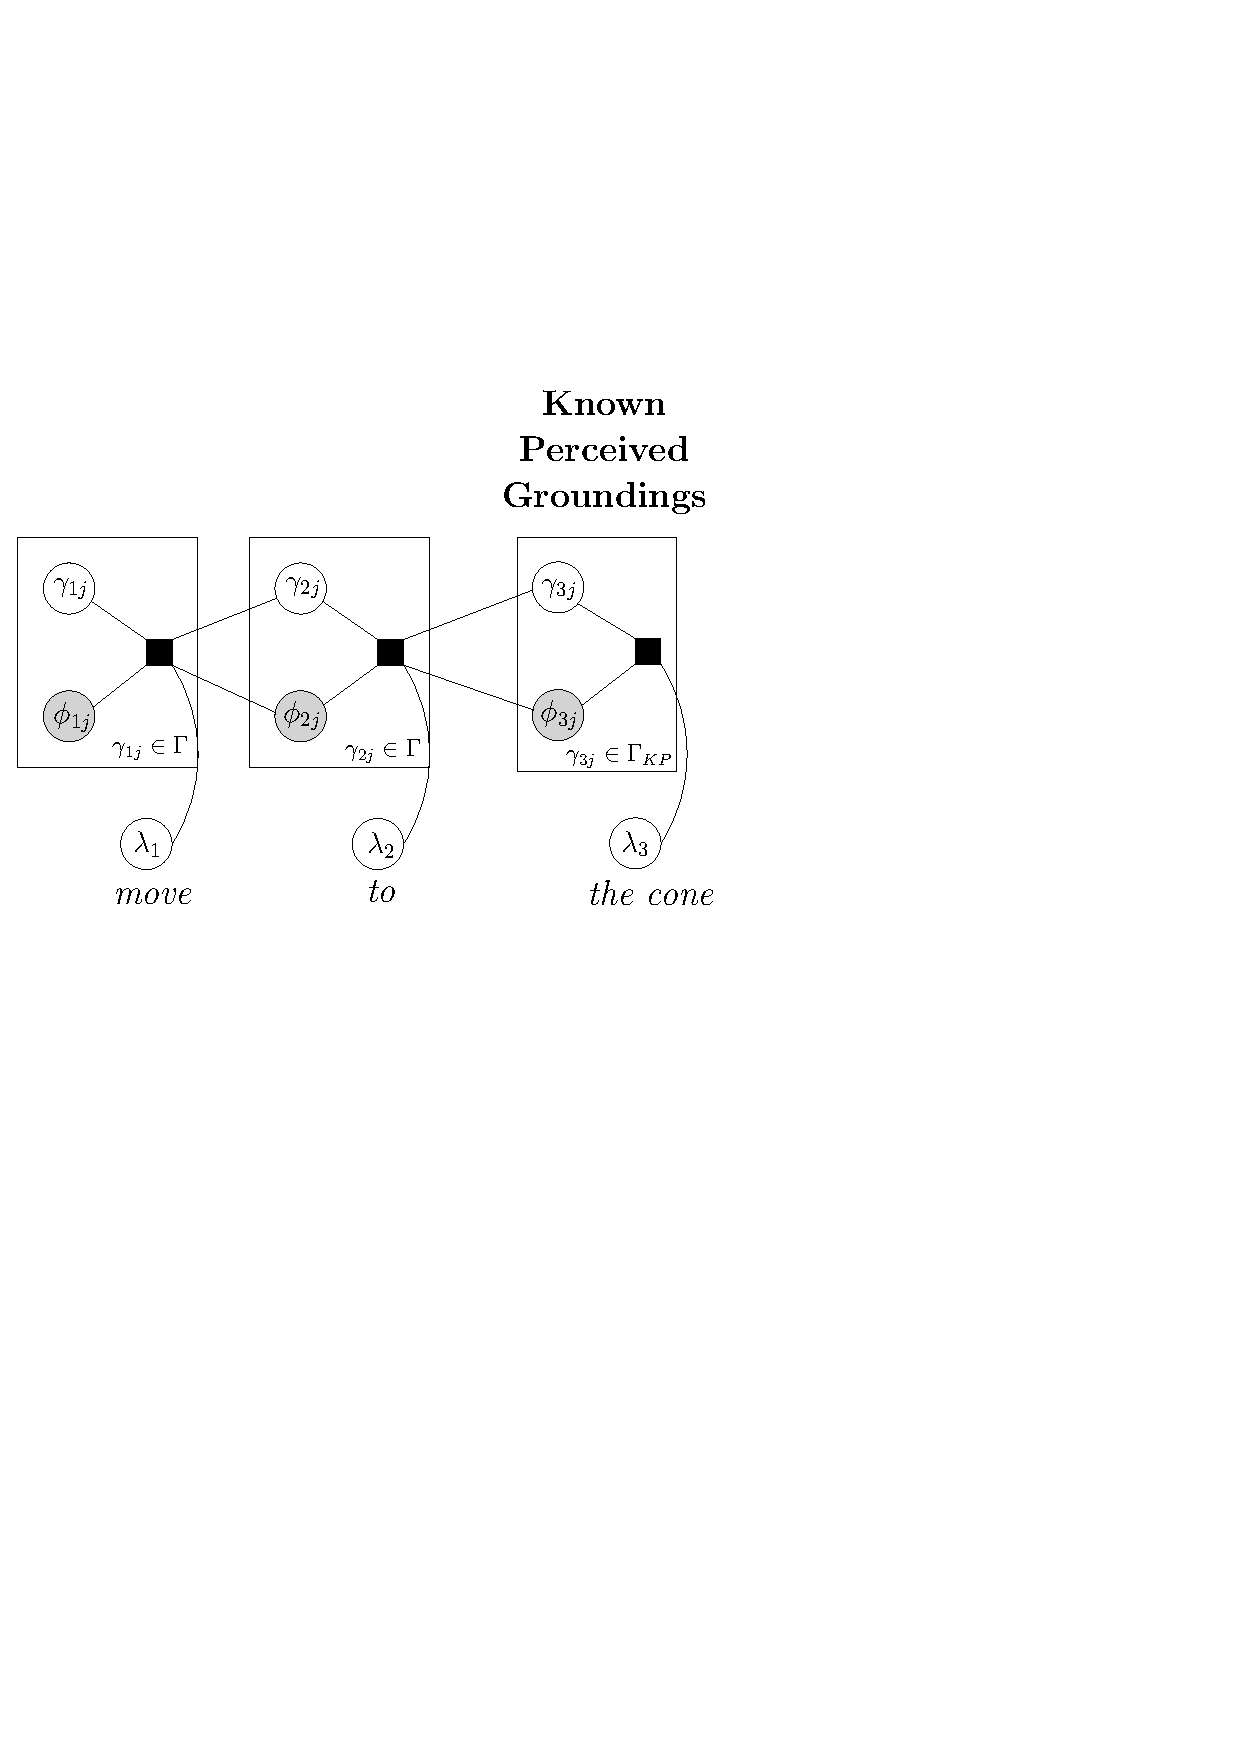
\includegraphics[width=\textwidth]{dcg.pdf}
\caption{The DCG model}
\end{subfigure}
~
\begin{subfigure}[t]{0.31\textwidth}
\centering
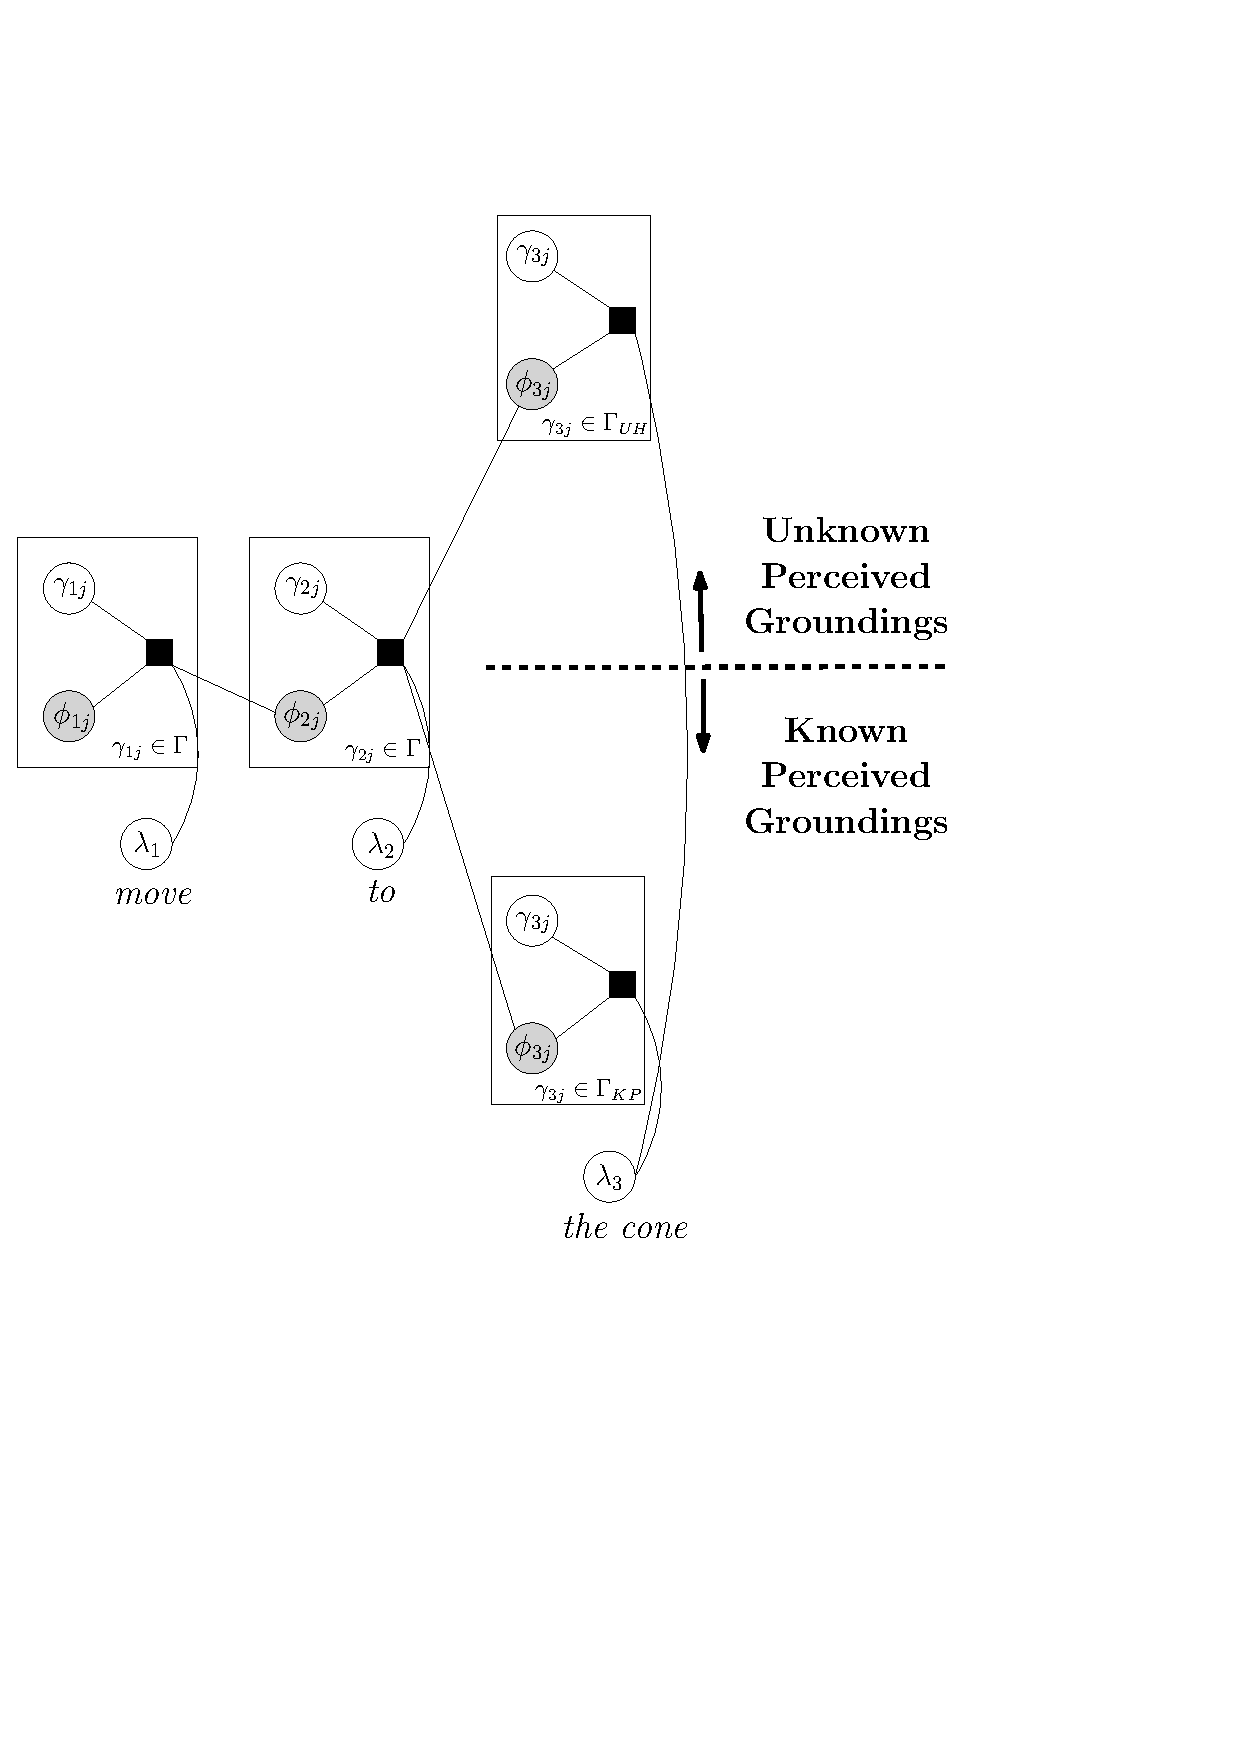
\includegraphics[width=\textwidth]{dcg_upup.pdf}
\caption{The DCG-UPUP model}
\end{subfigure}
~
\begin{subfigure}[t]{0.4\textwidth}
\centering
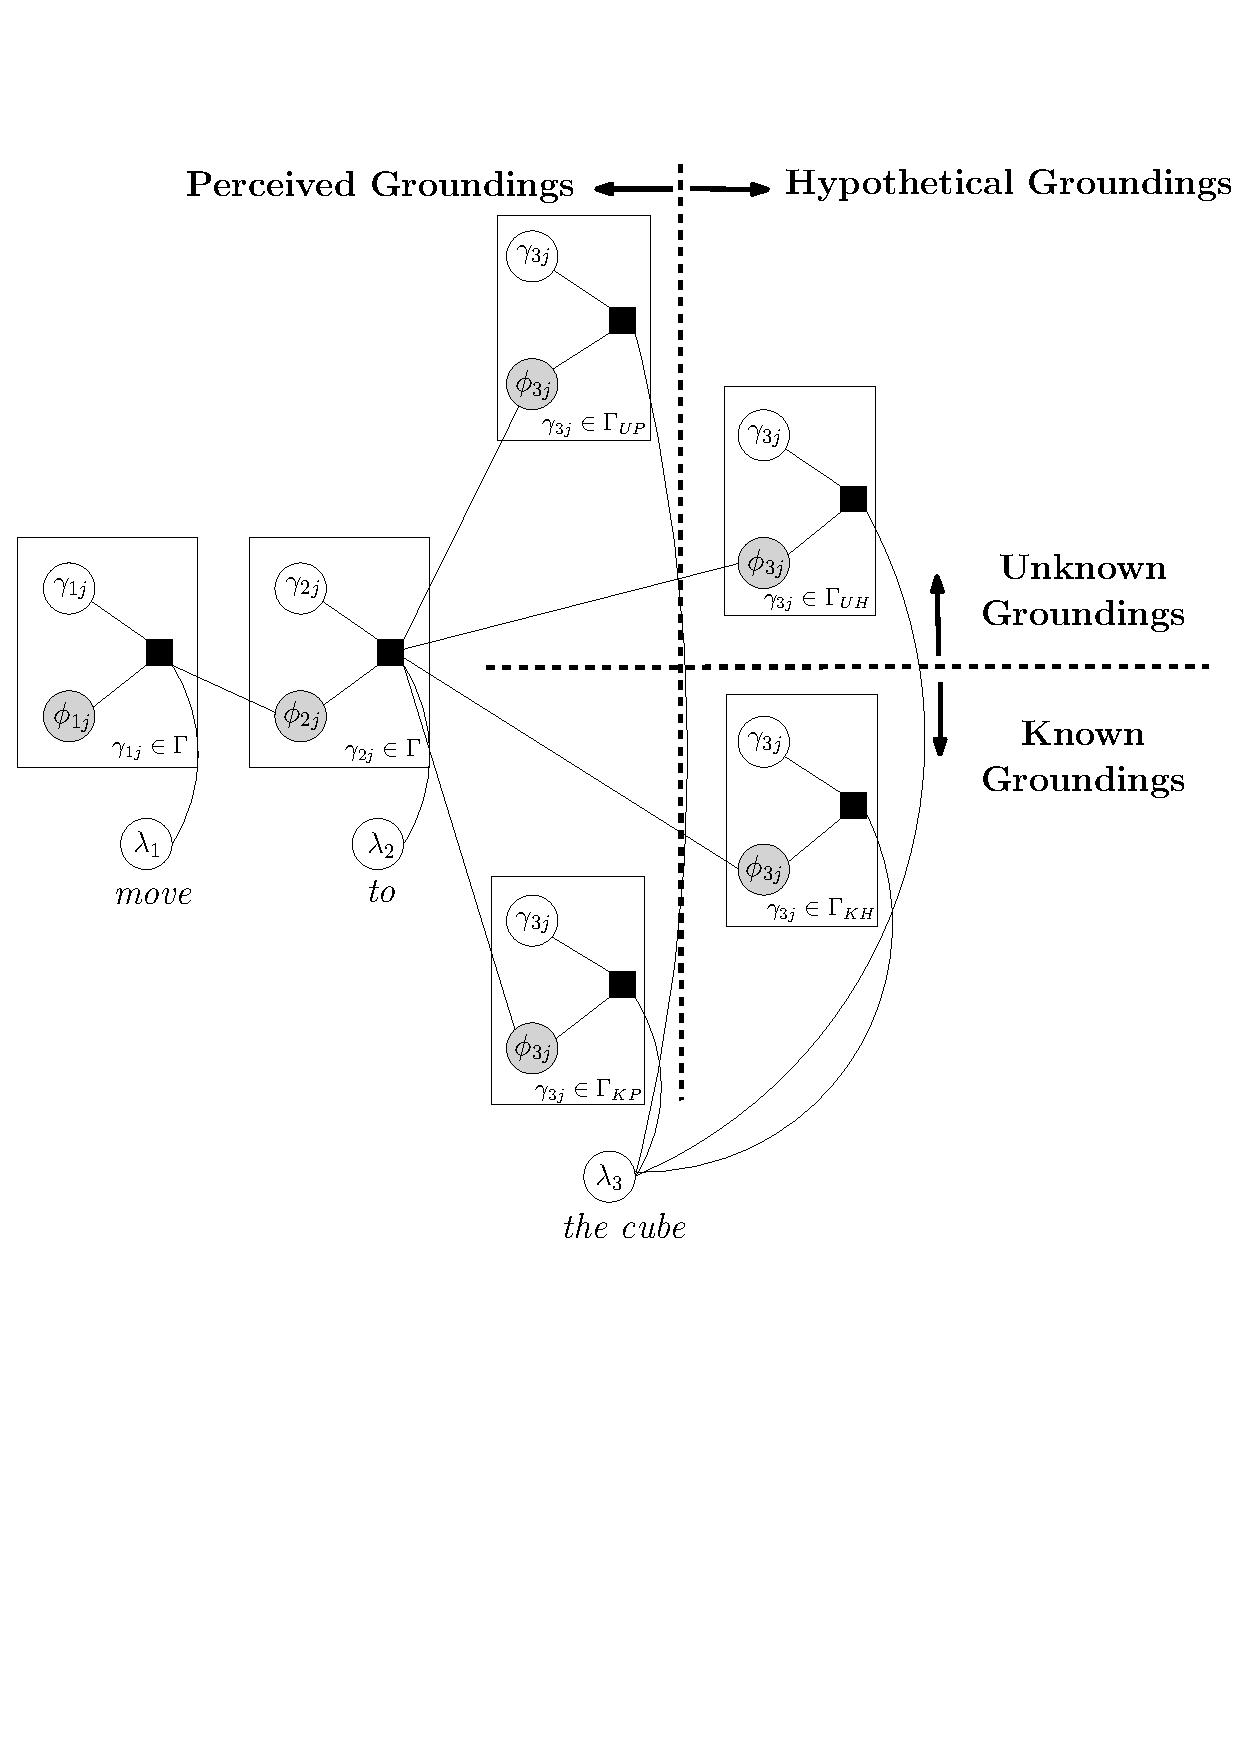
\includegraphics[width=\textwidth]{dcg_upup_away.pdf}
\caption{The DCG-UPUP-Away model}
\end{subfigure}
\caption{The graphical models constructed for the command ``\emph{move to the cone}".}
\end{figure*}

\begin{figure}
\centering
\begin{subfigure}[t]{0.47\columnwidth}
\centering
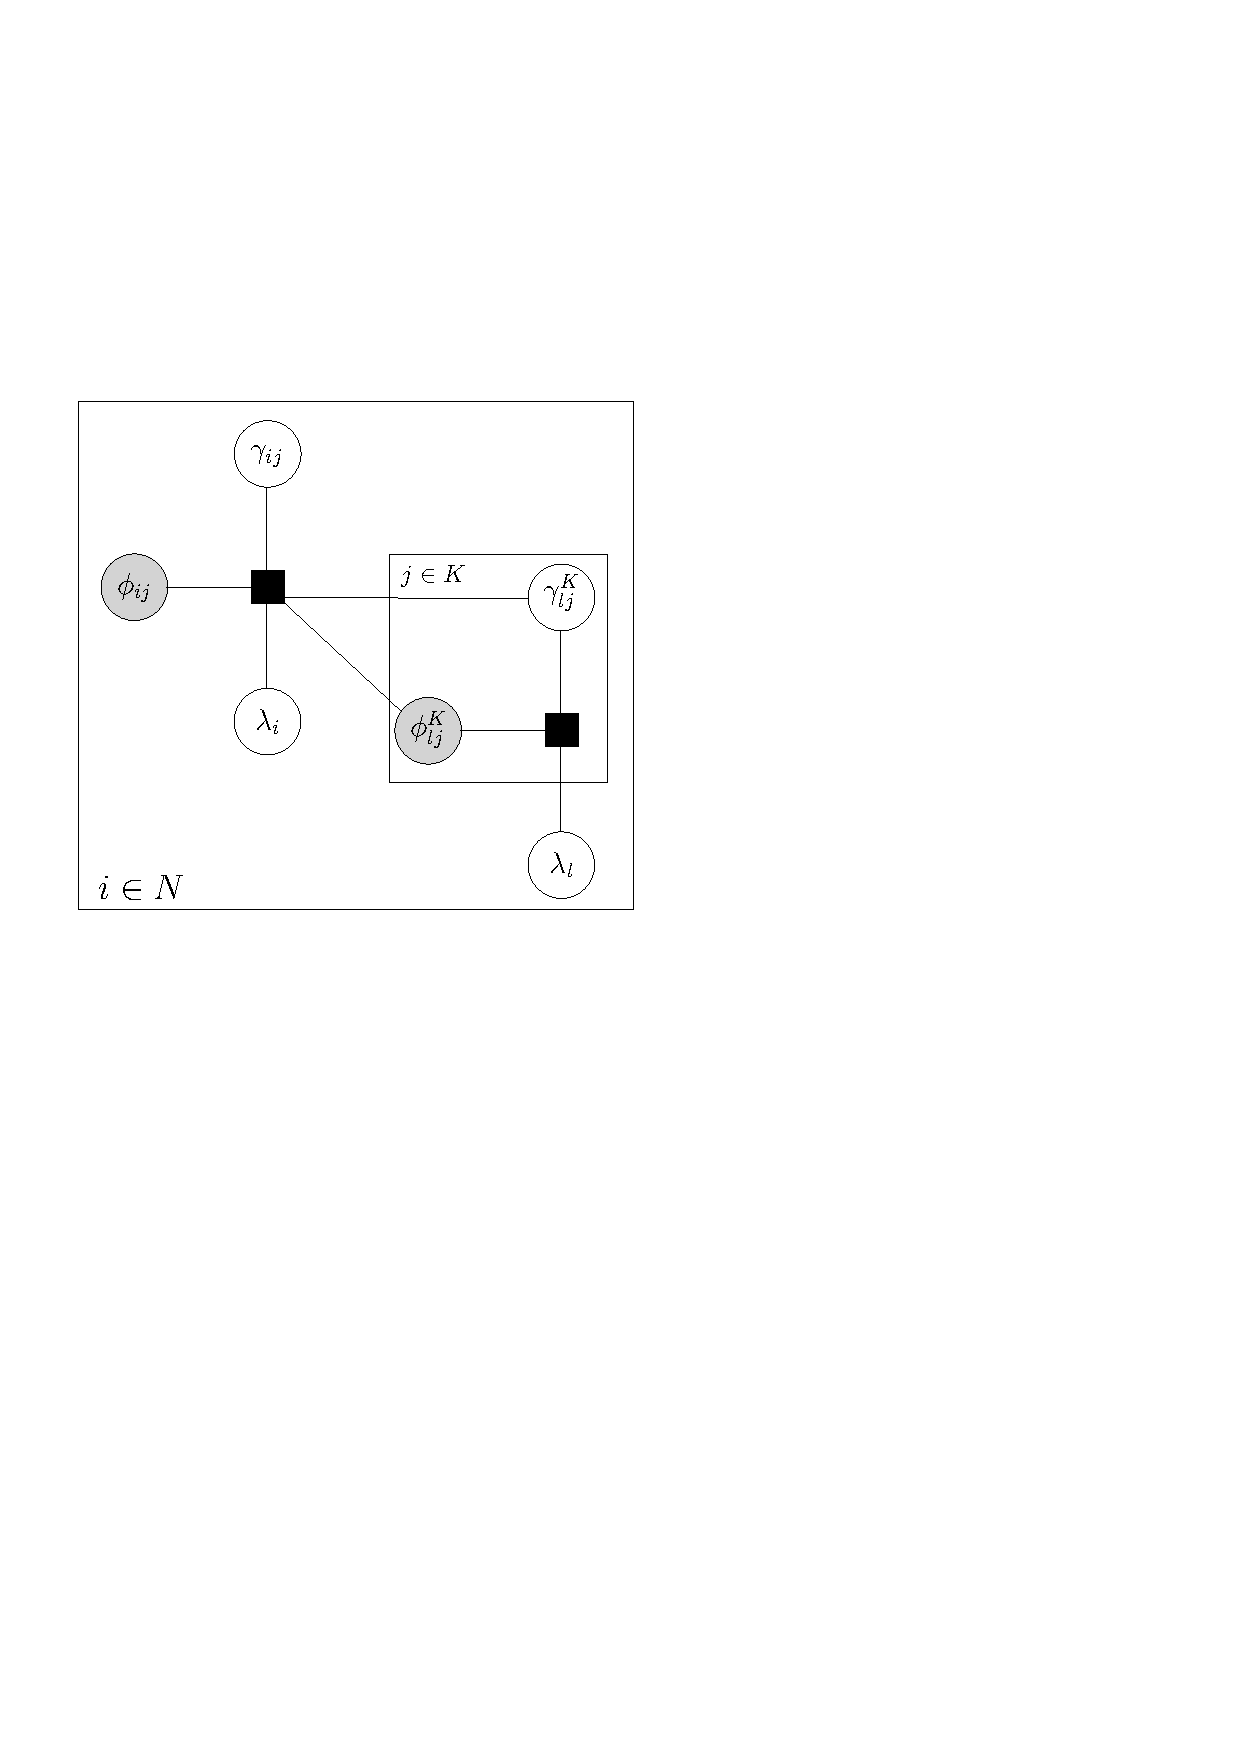
\includegraphics[width=\textwidth]{case1.pdf}
\caption{Without explicit unknown symbols}
\end{subfigure}
~
\begin{subfigure}[t]{0.49\columnwidth}
\centering
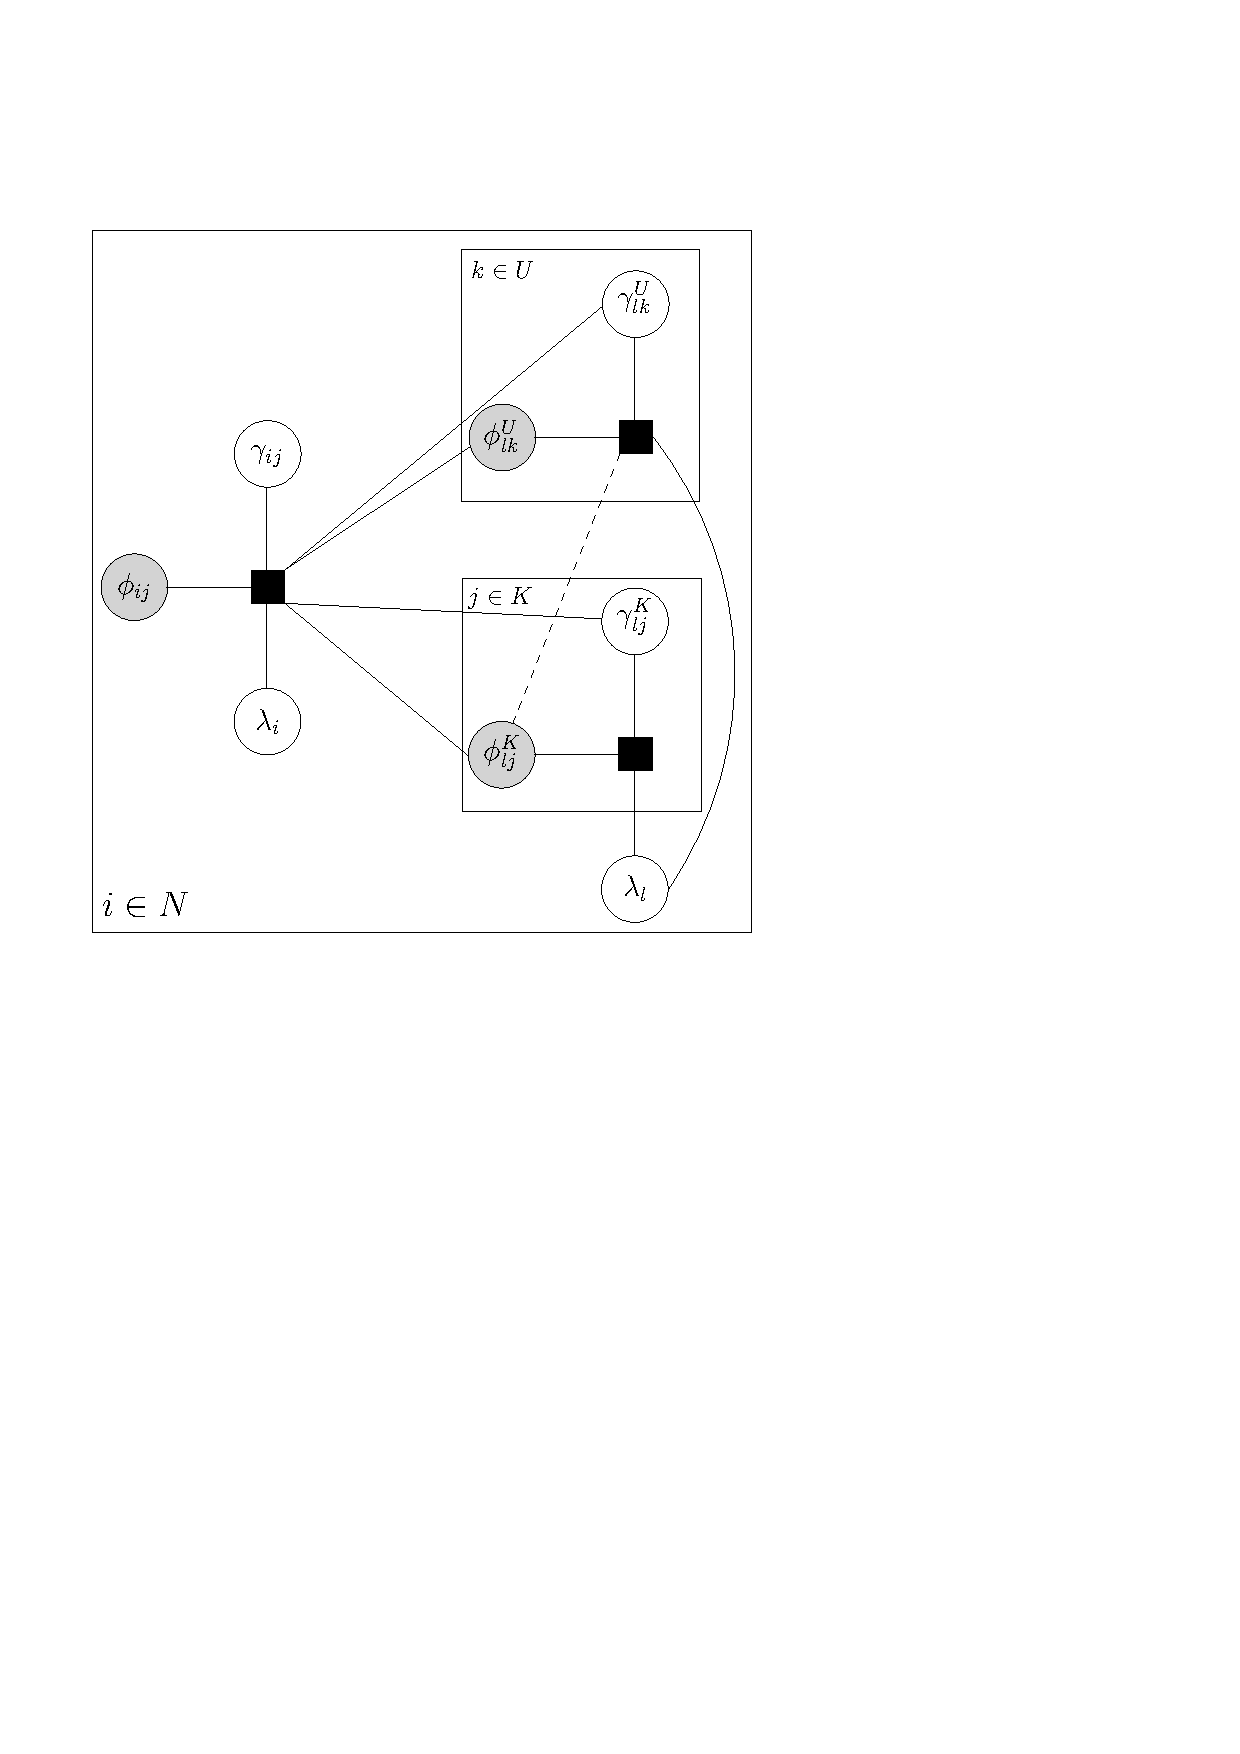
\includegraphics[width=\textwidth]{case2.pdf}
\caption{With explicit unknown symbols}
\end{subfigure}

\caption{Factor graph representations. Input instruction is parsed into $N$ phrases where $\lambda_l$ represents a child phrase of parent phrase $\lambda_i$. Superscripts $K$ and $U$ denote known and unknown variables, respectively.}
\end{figure}



\subsection{Adjective-Attribute Heuristics}
Here I describe how color can be used to bias the correct grounding.

Here are the equations.
The factored equation is the same as before, so I will leave it out.
The features:
\begin{equation}
\Psi() = \exp \Big( \sum_{f \epsilon F_{\text{DCG}}} \mu_f f(\phi_{ij},\gamma_{ij},\lambda_i,\Gamma_{c_{ij}},\Upsilon_{KP} \cup \Upsilon_{UP} \cup \Upsilon_{KH} \cup \Upsilon_{UH}) +...\\
\sum_{f' \epsilon F_{\text{Unknown}}} \mu_{f'} f'(\phi_{ij},\gamma_{ij},\lambda_i,\Gamma_{c_{ij}},\Upsilon_{KP} \cup \Upsilon_{UP} \cup \Upsilon_{KH} \cup \Upsilon_{UH}) +...\\
\mu_{f_H} f_{H}(\phi_{ij},\gamma_{ij},\lambda_i,\Gamma_{c_{ij}},\Upsilon_{KP} \cup \Upsilon_{UP} \cup \Upsilon_{KH} \cup \Upsilon_{UH}) +...\\
\sum_{f'' \epsilon F_{\text{Color}}} \mu_{f''} f''(\phi_{ij},\gamma_{ij},\lambda_i,\Gamma_{c_{ij}},\Upsilon_{KP} \cup \Upsilon_{UP} \cup \Upsilon_{KH} \cup \Upsilon_{UH}) \Big)
\label{eq:color_llm2}.
\end{equation}